\part[5] El bloque A cae verticalmente desde una altura $h$. El bloque B
comienza en el reposo y se desliza sin fricción sobre un plano inclinado de
altura $h$. Los bloques son idénticos.

\textbf{¿Cuál bloque golpea el suelo con mayor rapidez?}

\begin{minipage}{0.3\textwidth}
    \begin{figure}[H]
        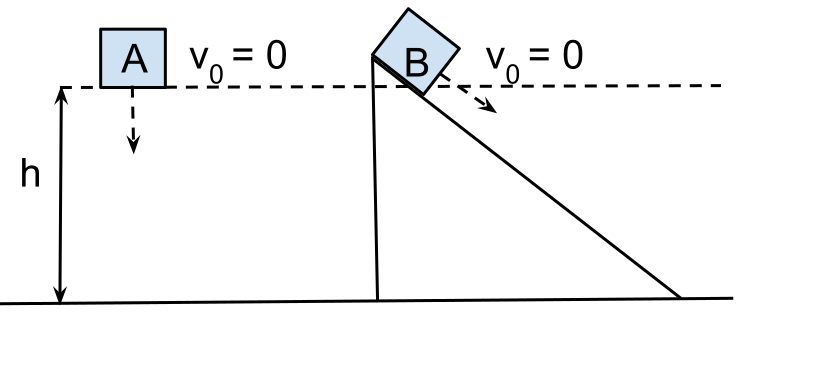
\includegraphics[width=\linewidth]{../images/f0bf197148397e9e0f833a29b1c58363c3a1ccb2}
    \end{figure}
\end{minipage}\hfill
\begin{minipage}{0.65\textwidth}
    \begin{choices}
        \choice El bloque A
        \choice No hay suficiente información
        \choice El bloque B
        \CorrectChoice Llegan al suelo con la misma rapidez
    \end{choices}
\end{minipage}